\documentclass[../main.tex]{subfiles}

\begin{document}

\subsection{Aim 2: Query Generation Methods Development and Evaluation}

In Aim 2 we focus on development and evaluation of methods for query generation and reasoning on eligibility criteria. We divide this aim into two sub-aims: (1) Development of a gold standard eligibility criteria logical forms corpus, and (2) Creation of methods for query generation utilizing the corpus in (1). This aim is largely complete and currently in the analysis phase.

\subsubsection{Related Work}

Various methods for matching eligibility criteria to cohorts of patients using NLP have been put forth by the research community \cite{yuan2019criteria2query, soni2020patient, fang2022combining, zhang2020deepenroll, chen2019clinical, patrao2015recruit, dhayne2021emr2vec, liu2021evaluating, xiong2019cohort}. NLP-based cohort discovery methods hold unique potential and appeal, as they are theoretically able to leverage existing eligibility criteria described in natural language, a medium researchers and investigators already use and are comfortable with. Recent methods which utilize NLP in some form can generally be grouped into 5 categories:

\begin{enumerate}
    \item{\textbf{Database query generation} to Structured Query Language (SQL) or similar systems using either (a) rules, (b) neural network-based encoder-decoder architectures}, or both.
    \item{\textbf{Document ranking and classification} using clinical notes in terms of relevancy vis-à-vis a given eligibility criteria.}
    \item{\textbf{Projection into embeddings} of patient medical history and trial eligibility criteria in a shared vector space and matching via similarity measurement or entailment.}
    \item{\textbf{Logical representations and reasoning} to represent eligibility criteria and patient records, matching by combinations of Semantic Web technologies, ontologies, Description Logics, and rule-based reasoning.}
    \item{A combination of the above.}
\end{enumerate}

\noindent Next we briefly describe recent relevant work in each category. \\

\textbf{Database query generation} - SQL-based relational databases are widely used both commercially and within academic institutions, and as such SQL is perhaps unsurprisingly often the target language in natural language to database query research \cite{dar2019frameworks}. Yuan \textit{et al} developed Criteria2Query, a hybrid information extraction (IE) pipeline and application which uses both rules and machine learning to generate database queries on an OMOP database. This work was expanded by Fang \textit{et al}, who added functionality for iterative query generation via human correction and adjustment \cite{fang2022combining}. Although not specific to RCTs, other highly relevant recent work on query generation in the biomedical domain has been done using Encoder-Decoder neural architectures for transforming clinical natural language questions into SQL queries \cite{bae2021question, park2021knowledge, wang2020text, pan2021bert, dhayne2021emr2vec}. Park \textit{et al} \cite{park2021knowledge} experimented with transforming medical questions generated in the MIMICSQL data set \cite{johnson2016mimic, wang2020text} using both SQL and SPARQL queries with varying database schema representations. Bae \textit{et al} similarly experimented with methods for handling typos, misspellings, and abbreviations in generating SQL queries from natural language questions. Pan \textit{et al} \cite{pan2021bert} leveraged intermediate abstract syntax tree-based representations and a SQL grammar-based Decoder architecture for dynamic database schema matching. 

\textbf{Document ranking and classification} - Focusing on clinical notes, Chen \textit{et al} \cite{chen2019clinical} used hybrid rule-based heuristics and sentence pattern-matching to detect criteria structure, as well as a combination of neural network-based bi-directional long short-term and conditional random field (biLSTM+CRF) architecture and knowledge graphs using the UMLS for determining condition, lab, procedure and drug relationships. Soni and Roberts \cite{soni2020patient} utilized the BERT Transformer architecture \cite{devlin2018bert} and Lucene \cite{lucene} to summarize, rank and classify clinical notes as relevant to a given eligibility criterion, with the most relevant notes predicted to be eligible. 

\textbf{Embedding projections} - Dhayne \textit{et al} \cite{dhayne2021emr2vec} experimented with treating patient-to-RCT matching as a joint embedding and similarity measurement problem while also incorporating the SNOMED-CT ontology to infer basic "is-a" and "has-type" relations between concepts. Similarly, Zhang \textit{et al} \cite{zhang2020deepenroll} used joint patient and eligibility criteria embeddings for entailment prediction, where predicting that a patient can be inferred from a given eligibility criteria equates to eligibility. 

\textbf{Logical representations and reasoning} - Patrao \textit{et al} developed Recruit \cite{patrao2015recruit}, an ontology-driven trial recruitment system which transformed SQL relational data to Resource Description Framework (RDF) graph-based triples. The RDF triples in turn were made query-able by use of an OWL-based reasoning system \cite{owl} and normalization techniques to infer cancer staging. Building upon earlier work \cite{patel2007matching, tu2009ergo, huang2013semanticct}, Baader \textit{et al} \cite{baader2018patient} explored the use of Description Logics and ontologies in matching patients in the MIMIC data set to logical representations of eligibility criteria, for example representing "Diabetes mellitus type 1" as "$\exists_y$.diagnosed\_with(x, y) $\wedge$ Diabetes\_mellitus\_type\_1(y)". Liu \textit{et al} \cite{liu2021evaluating} used domain experts to manually translate criteria into a custom syntax parsable by software. For example, the criterion "Patients more than 18 years old when they received the treatment" would be represented as "\#Inclusion features['StartDate'] >= demographics['BirthDate'] + @YEARS(18)". Parsed eligibility criteria were then executed on a proprietary database schema to determine eligible patients.

\subsubsection{Sub-Aim 1: Creation of a Criteria to Logical Form Gold Standard}

Query generation for LeafAI was originally envisioned as a system which generates queries using rules executed upon predicted named entities and relations in the form of graphs. In practice, we found this system to be difficult to manage given the need for ever more rules, as well as error-prone in handling new unseen criteria, which in turn required the creation of additional rules.

As a solution to this, we instead explored the transformation of  eligibility criteria into intermediate "logical form" representations, then generating SQL statements from the parsed logical forms. Intermediate representations (IRs) have a long history in computer science and NLP. IRs remove "noise" unnecessary to a given task and more closely represent underlying semantics while being agnostic to particulars of a final executed form (see Herzig \textit{et al} \cite{herzig2021unlocking} for an examination of IR-based SQL generation approaches). In related work, Roberts and Demner-Fushman \cite{roberts2016annotating} proposed an IR of questions on EHR databases using a comparatively compact but flexible format using first order logic expressions, for example, representing "Is she wheezing this morning?" as

\begin{quote}
    \centering
    $\delta( \lambda x.has\_problem(x, C0043144, status) \wedge time\_within(x, \mathrm{"this\ morning"}))$
\end{quote}

\noindent This style of representation is highly generalizable, but also difficult to translate directly into SQL statements as multiple predicates (e.g., \textit{has\_problem} and \textit{time\_within}) may correspond to a variable number of SQL statements, depending on context.

We thus chose a similar IR (hereafter simply "logical form") as proposed by Roberts and Demner-Fushman but closely more resembling a nested functional structure in programming languages such as Python or JavaScript. A criterion such as "Diabetic women and men over age 65" would be represented by our logical forms as

\begin{quote}
$intersect( \\
    \mathrm{\ \ \ \ }cond("Diabetic"), \\
    \mathrm{\ \ \ \ }union(female(), male()),\\
    \mathrm{\ \ \ \ }age().num\_filter(eq(op(GT), val("65"))) \\
)$
\end{quote}

We named the corpus produced from this sub-aim the Leaf Logical Forms (LLF) corpus. We developed annotation guidelines for the LLF corpus using a simplification of entities and relations from the preceding LCT corpus discussed in Aim 1. Generally speaking, LCT \textit{entities} correspond to logical form \textit{functions}, while LCT \textit{relations} correspond to logical form \textit{predicates}. For example, the LCT \textit{Condition} entity has a corresponding \textit{cond()} function, while the \textit{Num-Filter} relation has a corresponding \textit{.num\_filter()} predicate. The LLF annotation guidelines can be found at \url{https://github.com/ndobb/clinical-trials-seq2seq-annotation/wiki}.

We also hypothesized that the performance of predicting logical forms could likely be improved by replacing "raw" tokens in each eligibility criteria with corresponding logical form names derived from named entities from the LCT corpus. For example, given the eligibility criterion: \\

"\textit{Diabetics who smoke}", \\

\noindent we would replace the named entities for "Diabetics" and "smoke": \\ 

\textit{cond("Diabetics") who obs("smoke")} \\

\noindent using \textit{Condition} and \textit{Observation} annotations in the LCT corpus. We call this substituted text an "augmented" eligibility criteria. The augmented criteria syntax reshapes named entities to more closely resemble expected logical form syntax and allows us to leverage the LCT corpus for logical form transformation.

Creation and annotation of the LLF corpus proceeded in the following steps:

\begin{enumerate}
    \item We randomly chose 2,000 lines of eligibility criteria from the LCT corpus, limited to only criteria which included at least one named entity and which were not annotated as hypothetical criteria.
    \item  Each annotation file consists of the text "EXC" if exclusion or "INC" if inclusion (line 1), an original "raw" eligibility criteria (line 3), an augmented eligibility criteria (line 5), and an (initially blank) expected logical form equivalent to annotate (line 7). An example annotation is shown in Figure \ref{aim2_annotation_example}.
    \item 3 informatics graduate students met weekly for 2 months to review annotations. Annotators were initially trained on 20 triple-annotated training annotations. 
    \item After training, each annotator was assigned a batch of 100 sentences (one per file) and tasked with writing a logical form version of each.
    \item After each batch was completed, we executed a quality control script to parse each logical form annotation to ensure consistency. Any syntax errors were reported to and corrected by the annotators.
    \item Annotators received additional batches of files to annotate until all 2,000 single-annotated annotations had been completed.
\end{enumerate}

\begin{figure}[h!]
  \centering
  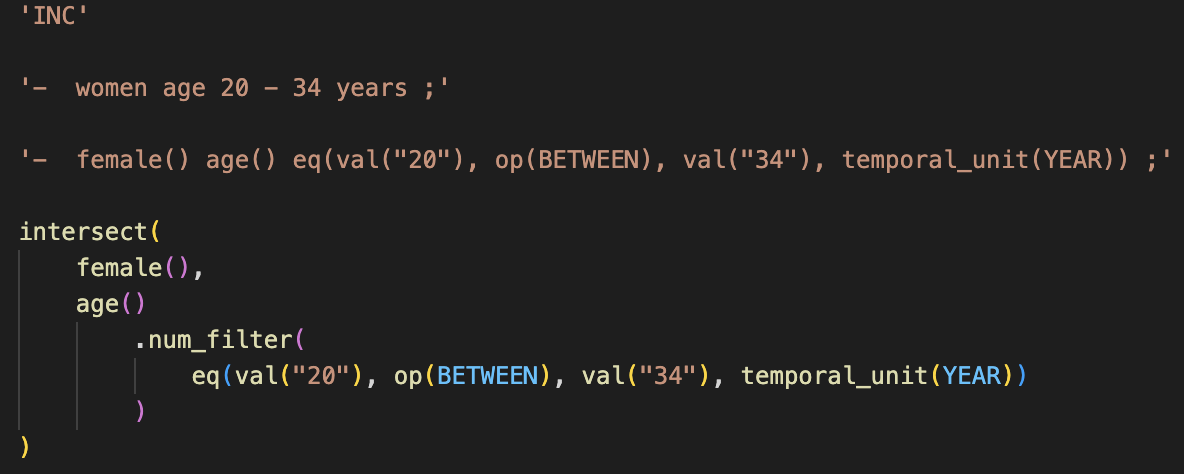
\includegraphics[scale=0.8]{Figures/Aim2/aim2_leafai_annotation_example.png}  
  \caption{A example LLF corpus annotation. The annotation file is saved in JavaScript (.js) format, which enables syntax highlighting and validation to assist annotators. Whether a given criterion was an inclusion or exclusion criteria is indicated at the top, followed by the original raw text, then augmented text. The final annotated logical forms are shown last.}
\label{aim2_annotation_example}
\end{figure}

After annotations were completed, we experimented with predicting logical forms by fine-tuning T5 \cite{raffel2020exploring} Seq2Seq models. The T5 architecture and pre-trained models are widely used for and achieve at or near state-of-the-art for many machine translation and semantic parsing tasks. 

Following earlier work on task-oriented dialog semantic parsing structures in the domain of digital assistants, we also experimented using various alternative input-output syntax styles from our original logical forms:

\begin{enumerate}
    \item \textbf{Shift-Reduce}. Einolghozatic \textit{et al} \cite{einolghozati2019improving} used square brackets instead of parentheses and blank spaces instead of commas. We followed Rongali \textit{et al's} suggestion to add a trailing repeat of function names to improve performance.
    \item \textbf{Pointer}. Rongali \textit{et al} found that replacing input tokens with "$@ptr_{index}$", where \textit{index} corresponds to a token's sequential position in the input text improved performance in their semantic parsing task. We modified this approach by omitting the characters "ptr" and using the sequential position of the quoted span as our index rather than individual token positions.
\end{enumerate}

We used a randomly sorted 70/20/10 train/test/validation split of the LFF corpus to fine-tune the pretrained T5$_{base}$ model using combinations of these syntax styles. We call our gold standard annotated logical form syntax "Standard" style. Example inputs, outputs, and training results are shown in Table \ref{aim2_tbl_corpus}. 

\begin{table}[h!]
    \footnotesize
    \centering
    \def\arraystretch{1.4}
\definecolor{gray}{RGB}{230,230,230}
\begin{tabular}{m{2.5cm} l l l l}
    \toprule
    \textbf{Syntax Style} & \textbf{Example Input} & \textbf{Example Logical Form} & \textbf{BLEU} & \textbf{ROUGE-L} \\
    \midrule
    \arrayrulecolor{gray}
    Raw-text→ Standard       
       & Diabetics who smoke                     
       & $\makecell[cl]{intersect(\\\mathrm{\ \ \ }cond("Diabetics"), \\\mathrm{\ \ \ }obs("smoke")\\)}$
       & 78.7
       & 79.1 \\
    \midrule
    Standard  
       & cond("Diabetics") who obs("smoke")           
       & $\makecell[cl]{intersect(\\\mathrm{\ \ \ }cond("Diabetics"), \\\mathrm{\ \ \ }obs("smoke")\\)}$
       & \textbf{94.4}
       & \textbf{91.5} \\
    \midrule
    Standard+ Pointer
       & cond(@1) who obs(@2)                          
       & $\makecell[cl]{intersect(\\\mathrm{\ \ \ }cond(@1), \\\mathrm{\ \ \ }obs(@2)\\)}$
       & 93.3
       & 91.2 \\
    \midrule
    Shift-Reduce              
       & [cond "Diabetics" cond] who [obs "smoke" obs] 
       & $\makecell[cl]{[intersect\\\mathrm{\ \ \ }[cond\mathrm{\ }"Diabetics"\mathrm{\ }cond]\\\mathrm{\ \ \ }[obs\mathrm{\ }"smoke"\mathrm{\ }obs]\\ intersect]}$
       & 89.8
       & 91.7 \\
    \midrule
    Shift-Reduce+ Pointer     
       & [cond @1 cond] who [obs @2 obs]               
       & $\makecell[cl]{[intersect\\\mathrm{\ \ \ }[cond\mathrm{\ }@1\mathrm{\ }cond]\\\mathrm{\ \ \ }[obs\mathrm{\ }@2\mathrm{\ }obs]\\ intersect]}$
       & 89.4
       & 90.4 \\
    \bottomrule       
\end{tabular}
    \caption{Example inputs and logical form syntax styles with fine-tuning performance results using the T5$_{base}$ model.}
    \label{aim2_tbl_corpus}
\end{table} 

We found that our Standard logical forms achieved the highest performance using both BLEU \cite{lin2004rouge} and ROUGE-L \cite{callison2006re} scores, two commonly used metrics in measuring Seq2Seq performance. Replacing raw tokens with function names corresponding to named entities also significantly improved performance (+14.7\%, comparing raw text to Standard input styles), demonstrating that leveraging the LCT corpus to generate augmented text achieved relatively high performance (> 93\% BLEU score) for this task. As it was the highest-performing syntax style and also the most straightforward to parse, we chose to use the Standard logical form style as our IR for our work in sub-aim 2.

\subsubsection{Sub-Aim 2: Query Generation}
In sub-aim 2, we developed the LeafAI query engine, an application capable of generating database queries for cohort discovery from free-text eligibility descriptions. This sub-aim contributes the following:

\begin{enumerate}
    \item{A novel database schema annotation and mapping method to enable data model-agnostic query generation from natural language.}
    \item{Methods for transforming and leveraging intermediate logical representations of eligibility criteria.}
    \item{Methods for dynamically reasoning upon non-specific criteria using an integrated knowledge base of biomedical concepts.}
\end{enumerate}

\subsubsection{System Architecture}

The LeafAI query engine was designed using a modular, micro service-based architecture with a central API (Application Program Interface) which orchestrates end-to-end query generation. Inter-module communication is performed using gRPC \cite{grpc}, a robust open-source remote procedure call framework which enables language-agnostic service integration. This allows individual modules to be implemented (and substituted) in programming languages and using libraries well-suited to a given task. A diagram of the LeafAI query engine architecture is shown in Figure \ref{aim2_fig_leafai_architecture}. 

\begin{figure}[h]
  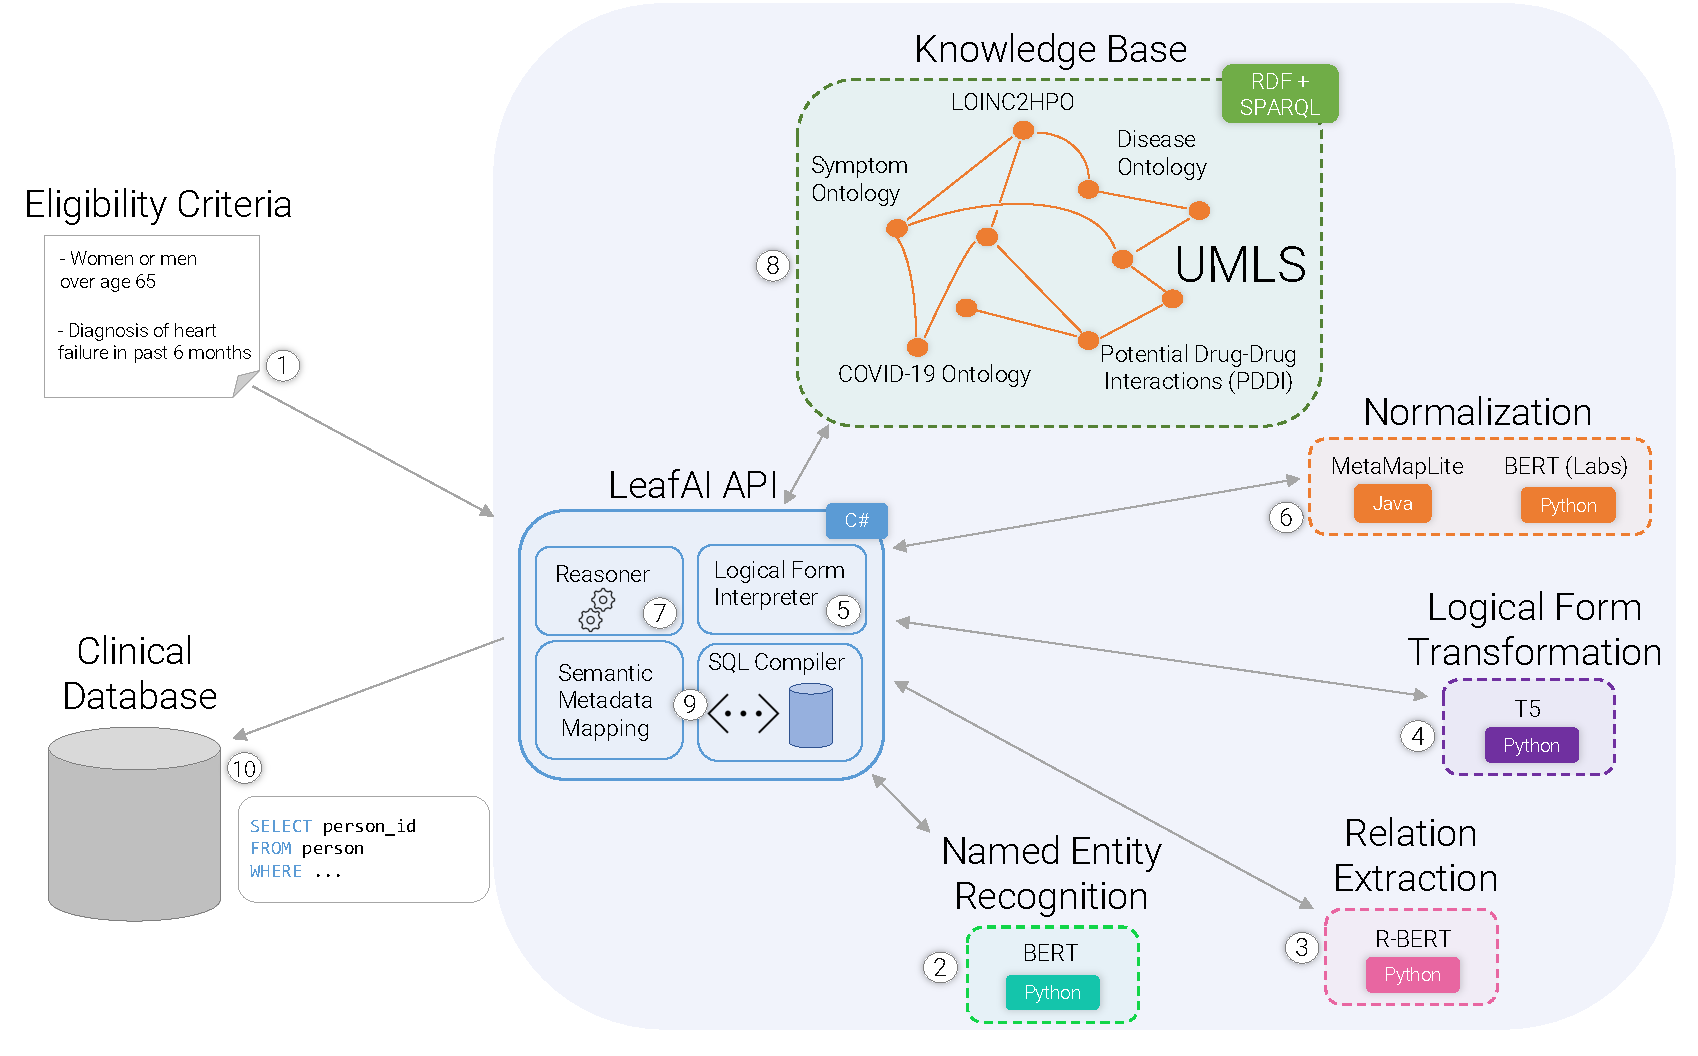
\includegraphics[scale=0.65]{Figures/Aim2/aim2_leafai_architecture.pdf}  
\caption{LeafAI query architecture. Inter-module communication is performed using the gRPC framework. Individual modules are deployed as Docker \cite{docker} containers and communicate solely with the central API, which orchestrates query generation and handles query generation requests.}
\label{aim2_fig_leafai_architecture}
\end{figure}

At a high level, query generation is performed in the following steps:

\begin{enumerate}
    \item{A query request is received by the API in the form of inclusion and exclusion criteria as free-text strings.}
    \item{The input texts are tokenized and named entity recognition is performed to determine spans of text representing conditions, procedures, and so on.}
    \item{Relation extraction is performed to determine relations between named entities. Any entities found with a hypothetical \textit{Assertion} relation (e.g., "could become pregnant") are excluded.}
    \item{The input eligibility criteria are transformed by replacing spans of "raw" text with logical form names as in sub-aim 1. The resulting augmented criteria are inputted into our fine-tuned T5 model, which outputs a predicted logical form string.}
    \item{A logical form interpreter module implemented as a recursive descent parser \cite{johnstone1998generalised} reads the logical form string and instantiates it as an abstract syntax tree (AST) of nested in-memory logical form objects.}
    \item{"Named" logical form objects (i.e., specified with quoted text, such as \textit{lab("hemoglobin A1c")}) are normalized into one or more corresponding UMLS concepts.}
    \item{Working recursively inside-to-outside the AST structure, each logical form object calls a \textit{Reason()} method which executes various rules depending on context.}
    \item{Each reasoning rule is performed as one or more pre-defined SPARQL queries to the knowledge base (KB), concept by concept.}
    \item{The normalized, reasoned, logical form AST is thus a nested structure of UMLS concepts. Each AST criterion is mapped to zero or more corresponding entries in the semantic metadata mapping (SMM).}
    \item{The final mapped AST object is transformed into a series of database queries, one per line of eligibility criteria text. The output SQL query can either be executed directly on a database or returned to the API caller.}
\end{enumerate}

\noindent Figure \ref{aim2_fig_leafai_querygen} illustrates an example of this process. Next we examine these steps in detail. \\

\begin{figure}[h]
  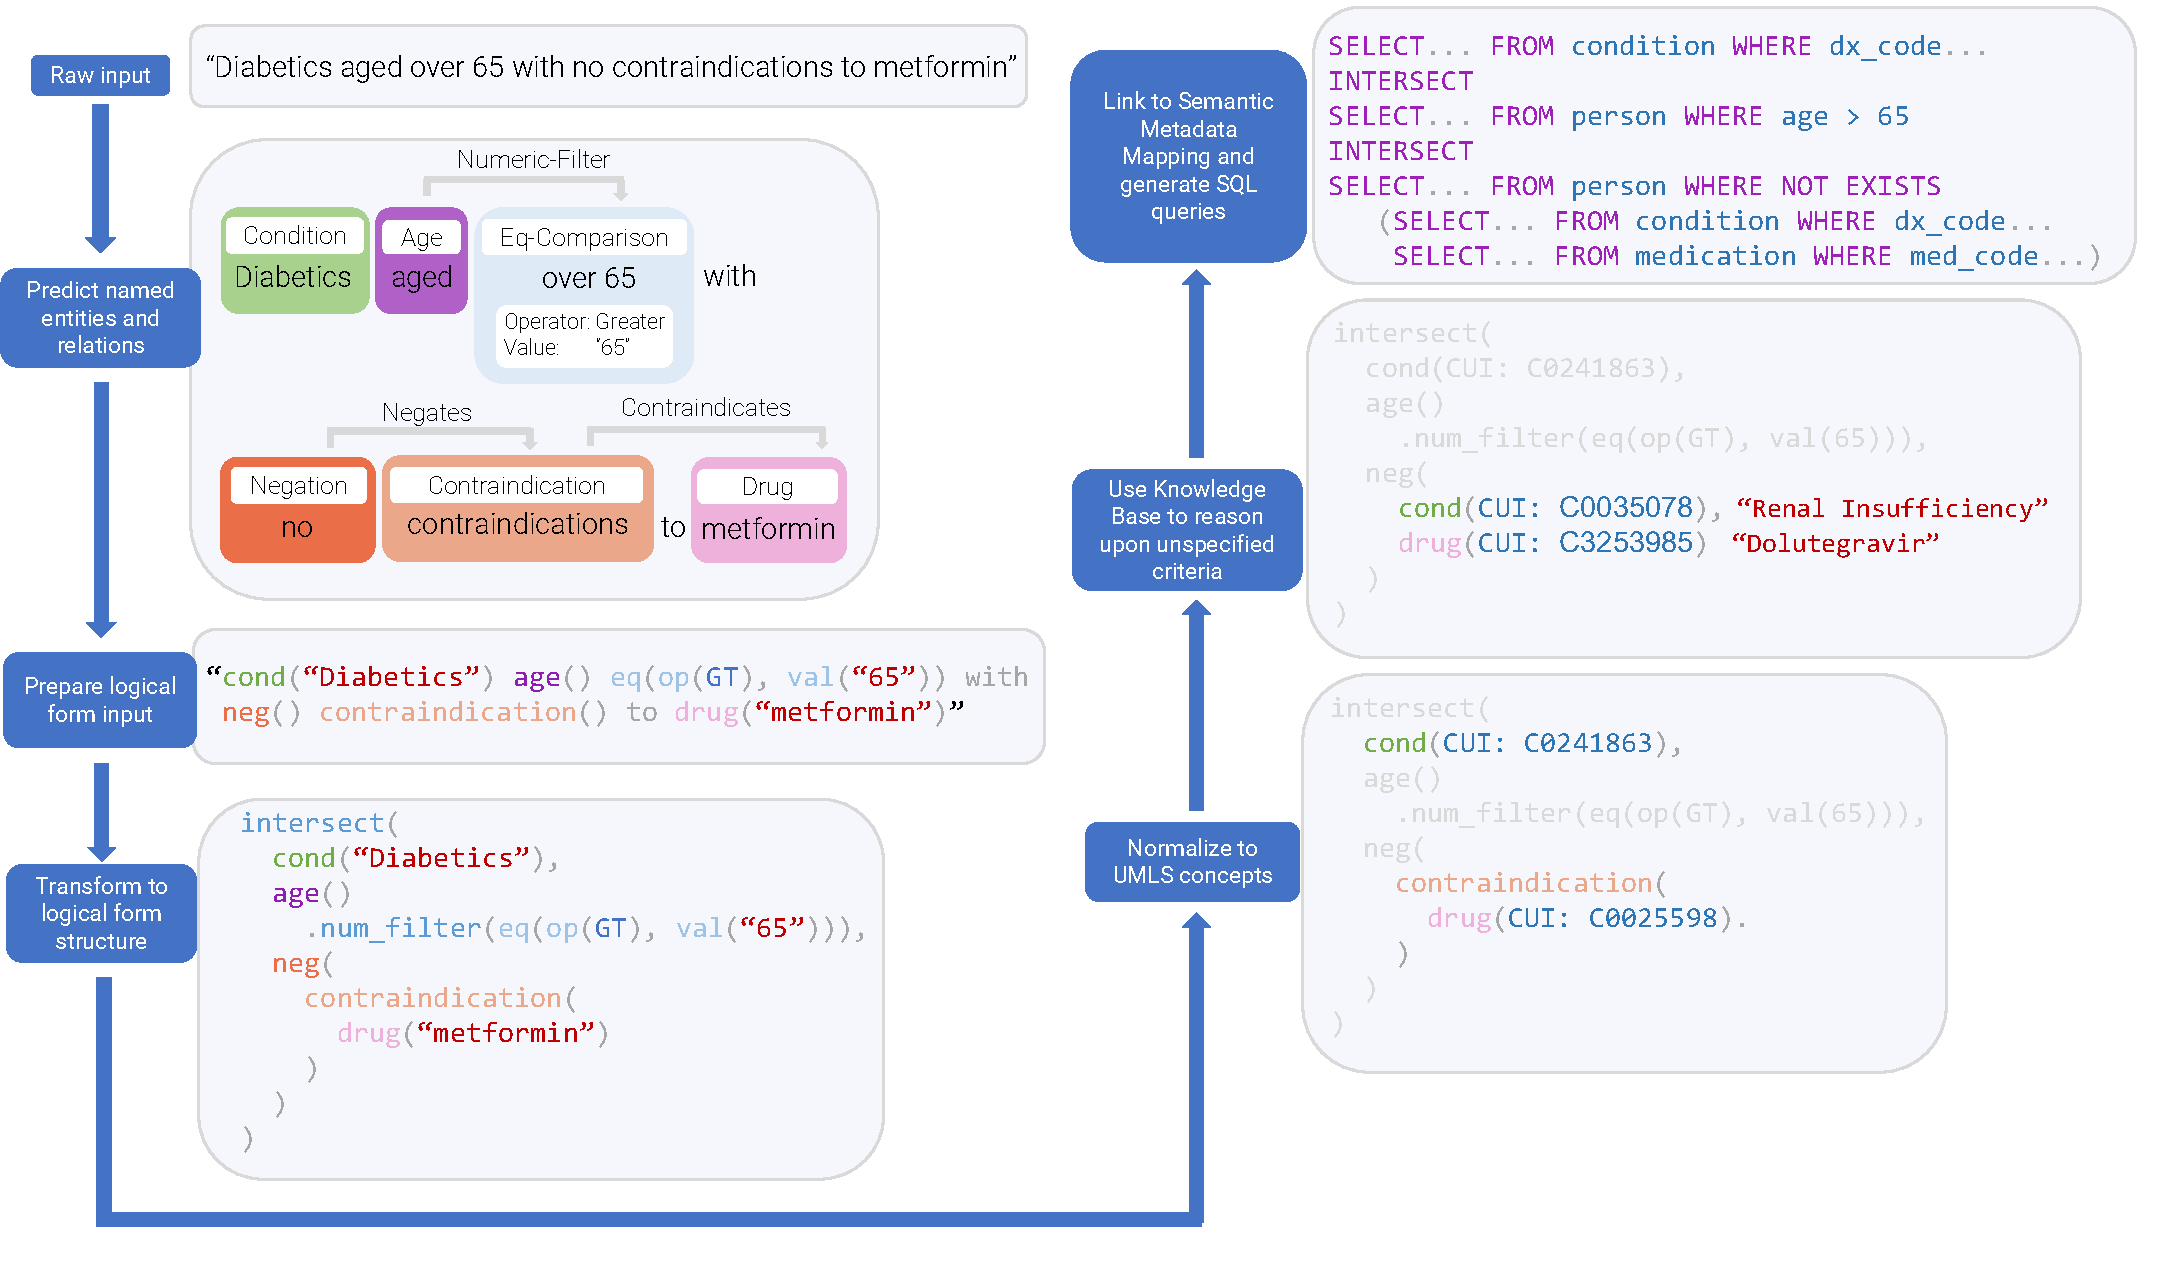
\includegraphics[scale=0.52]{Figures/Aim2/aim2_leafai_flow.pdf}  
\caption{LeafAI query generation processes}
\label{aim2_fig_leafai_querygen}
\end{figure}

\noindent \textbf{Named entity recognition and relation extraction} \\
We use the Leaf Clinical Trials (LCT) corpus \cite{dobbins2022leaf} to train two BERT-based \cite{devlin2018bert} NER extractors, one each for LCT general- and fine-grained-entities. Next, we perform relation extraction by enumerating named entity pairs similarly using a BERT-based model also trained on the LCT corpus. \\

\noindent \textbf{Logical form transformation} \\
As described in Sub-Aim 1, we leverage a fine-tuned T5 model for predicting logical forms. As inputs to the T5 model we use augmented text generated using predicted named entities. After prediction, the output logical form string is then instantiated into an AST of nested in-memory logical form objects using a recursive descent parser within the API. \\

\noindent \textbf{Concept normalization} \\
We consider a logical form "named" if it contains a free-text value surrounding by quotes. For logical forms besides laboratory values, we used MetaMapLite \cite{aronson2001effective, demner2017metamap}. Normalization using MetaMapLite can often result in high recall but low precision, as MetaMapLite matches potential candidate concepts across the UMLS. To improve normalization precision, we employ two strategies. First, we compare term frequency-inverse document frequency (tf-idf) on MetaMapLite predictions, dropping UMLS concepts whose matched spans have a tf-idf score lower than that of unmatched spans in a given named entity. For example, for the string "covid-19 infection", MetaMapLite predicts both "COVID-19" (C5203670) as well as several concepts related to general infections. Using our tf-idf strategy removes the erroneous infection concepts. Next, our NER component also us to further improve precision by filtering the predicted UMLS concepts to only those of specific semantic types. For example, we limit condition concepts to only those which include semantic types of signs or symptoms, diseases or syndromes, and so on. 

Laboratory values also present a particular challenge, as LeafAI requires lab concepts to have directly associated LOINC codes, while MetaMapLite typically normalizes lab test strings to UMLS concepts of semantic type "laboratory test or finding", but which do not have direct mappings to LOINC. For example, a search for "platelet count" with MetaMapLite returns the concept "Platelet Count Measurement" (C0032181), but not the needed concept of "Platelet \# Bld Auto" (C0362994). Thus similar to Lee and Uzuner with medications \cite{lee2020normalizing}, we trained a BERT model specifically for normalization of lab tests. \\

\noindent \textbf{Reasoning using an integrated knowledge base} \\
\noindent For reasoning and derivation of ICD-10, LOINC, and other codes for UMLS concepts, we designed a knowledge base (KB) accessible via SPARQL queries and stored as RDF triples. The core of our KB is the UMLS, derived using a variation of techniques created for ontologies in BioPortal \cite{noy2009bioportal}. To further augment the UMLS, we mapped and integrated the Disease Ontology \cite{schriml2012disease}, Symptom Ontology \cite{sayers2010database}, COVID-19 Ontology \cite{sargsyan2020covid}, Potential Drug-Drug Interactions \cite{ayvaz2015toward}, LOINC2HPO \cite{zhang2019semantic}, and the Disease-Symptom Knowledge Base \cite{wang2008automated}. We then developed SPARQL queries parameterized by UMLS concepts for various scenarios which leveraged our KB, such as contraindications to treatments, symptoms of diseases, and so on. Using LOINC2HPO mappings further allows us to infer phenotypes by lab test results rather than diagnosis codes alone. For example, given the logical form \textit{cond("Hypercalcemia")}, our system will search for abnormally high lab results of calcium [mass/volume] (LOINC: 17861-6) in addition to diagnosis codes.

Together our KB, nested logical forms, and inside-to-outside normalization and reasoning enable "multi-hop" reasoning on eligibility criteria over several steps. For example, given the non-specific criterion "Contraindications to drugs for conditions which affect respiratory function", our system successfully reasons that (among other results),

\begin{enumerate}
    \item \textbf{Asthma} causes changes to \textbf{respiratory function}
    \item \textbf{Methylprednisolone} can be used to treat \textbf{asthma}
    \item \textbf{Mycosis} (fungal infection) is a contraindication to \textbf{methylprednisolone}
\end{enumerate}

\noindent These features allow LeafAI to reason upon fairly complex non-specific criteria. \\

\noindent \textbf{Query generation using semantic metadata mapping} \\
To enable database schema-agnostic query generation, we leverage a subset of codes within the UMLS in what we define as a semantic metadata mapping, or SMM. An SMM is described using JSON, and includes a listing of available databases, tables, columns, and so on. Critically, these database artifacts are "tagged" using UMLS concepts. An example of this can be seen in Figure \ref{aim2_fig_leafai_smm}, which shows strategies by which a given criterion can be used to generate schema-specific queries by leveraging different SMMs. In cases where the LeafAI query engine finds more than one means of querying a concept (e.g., two SQL tables for diagnosis codes), the queries are combined in a UNION statement.

\begin{figure}[h!]
  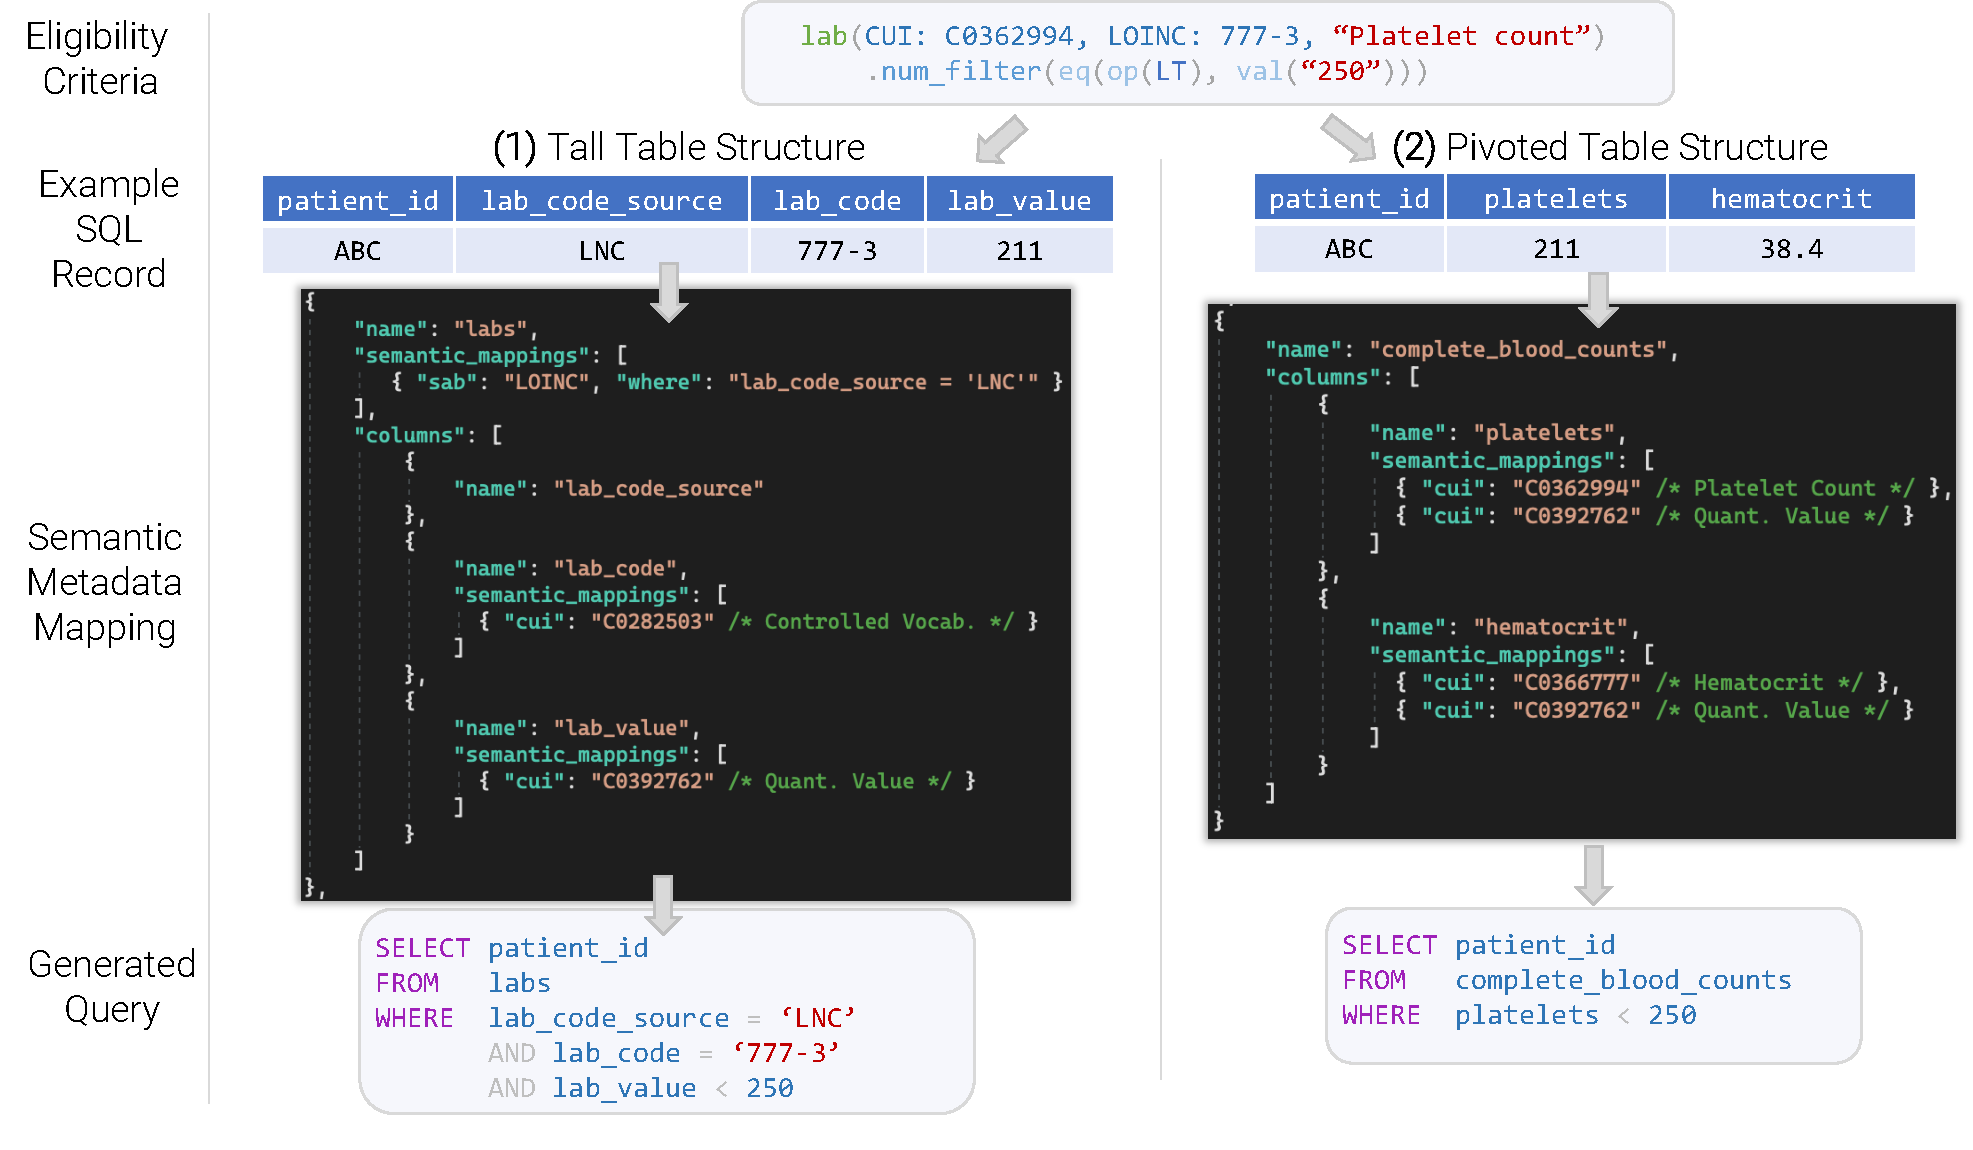
\includegraphics[scale=0.56]{Figures/Aim2/aim2_leafai_smm.pdf}  
\caption{The LeafAI query engine's SQL query generation process using two hypothetical database schema to generate queries for platelet counts (shown in logical form after normalization). This example illustrates the flexibility of LeafAI's semantic metadata mapping system in adapting to virtually any data model. On the left, "Tall Table Structure", platelet counts must be filtered from within a general purpose "labs" table. The LeafAI KB recognizes that labs may be stored as LOINC codes, and the corresponding SMM indicates that records in this table can be filtered to LOINC values. On the right, "Pivoted Table Structure", platelet counts are stored as a specific column in a "complete\_blood\_counts" table, and thus can be directly queried without further filtering. Additional metadata, columns, tables, types and so on needed in SMMs are omitted for brevity.}
\label{aim2_fig_leafai_smm}
\end{figure}

\subsubsection{Evaluation}
An NLP-based system for finding patients based on eligibility criteria should be reasonably expected to find many or most patients enrolled in a real clinical trial - with the assumption that patients enrolled in said trial correctly met the necessary criteria as determined by study investigators. While there are caveats to this approach (for example, certain structured data may be missing for some patients), we aimed to establish a new baseline by which tools such as ours are evaluated in their ability to handle real-world eligibility criteria and clinical data.

For comparison, we are analyzing database queries created by a human database programmer experienced with clinical databases and data extraction. Our evaluation is being performed as follows:

\begin{enumerate}
    \item We extracted metadata on 165 clinical trials from our EHR between January 2017 and December 2021 where at least 10 patients were indicated as enrolled and not withdrawn and the total number of raw lines within the eligibility criteria (besides the phrases "Inclusion Criteria" and "Exclusion Criteria") were less than or equal to 30. We excluded 41 trials with multiple sub-groups, as it would not be possible to know which eligibility criteria applied to which sub-group of enrolled patients.
    \item Using the "condition" field for each trial within metadata from \url{https://clinicaltrials.gov}, we filtered and grouped the remaining 124 trials into only those related to predetermined groups: Cardiology, COVID-19, Crohn's Disease, Multiple Sclerosis, Diabetes Mellitus, Hepatitis C, and Oncology. 
    \item We randomly chose 1 trial from each group, with the exception of Oncology, where we chose 2 trials.
    \item The human programmer was provided the eligibility criteria for each of the 8 selected trials and instructed to (1) ignore criteria which cannot be computed, (2) make a reasonable effort to reason upon non-specific criteria (e.g., symptoms for a condition), (3) not check whether patients found by a query enrolled within a trial, and (4) skip criteria which cause an overall query to find no eligible patients, as they typically indicate missing data.
    \item We generated queries using the LeafAI query engine, modifying the generated SQL to output the number of matched patients at each step. 
    \item In order to ensure results returned would be limited to only data available during the time of each trial, for each system we (1) replaced references to the SQL function for generating a current timestamp with that of each trial's end date, and similarly replaced OMOP table references with SQL views filtering data to only that existing prior to the end of a trial.
\end{enumerate}

\subsubsection{Results}

\begin{table}[h!]
    \footnotesize
    \centering
    \def\arraystretch{1.4}
\begin{tabular}{l l c c |r l |r l}
     & & & & \multicolumn{2}{c}{\textbf{LeafAI}} & \multicolumn{2}{|c}{\textbf{Human}}  \\
     \toprule
    \textbf{Condition} & \textbf{ID} & \textbf{Lines of Criteria} & \textbf{Enrolled} & \textbf{Matched} & \textbf{Eligible} & \textbf{Matched} & \textbf{Eligible} \\
    \midrule
    CLL                & \footnotesize{NCT04852822} & 4 & 83 & 80 (96\%) & 3,252 \\
    Hepatitis C        & \footnotesize{NCT02786537} & 8 & 42 & 33 (78\%) & 9,529 & 33 (78\%) & 4,981 \\
    Crohn's Disease    & \footnotesize{NCT03782376} & 9 & 16 & 0 (0\%) & 113 \\
    Cardiac Arrest     & \footnotesize{NCT04217551} & 12 & 27 & 12 (44\%) & 4,792 \\
    COVID-19           & \footnotesize{NCT04501952} & 13 & 41 & 0 (0\%) & 0 \\
    Multiple Sclerosis & \footnotesize{NCT03621761} & 14 & 196 & 149 (76\%) & 5,674 \\
    Type 1 Diabetes    & \footnotesize{NCT03335371} & 18 & 11  & 0 (0\%)      & 1,006 \\
    Ovarian Cancer     & \footnotesize{NCT03029611} & 25 & 11 & 10 (91\%) & 1,667 \\
    \bottomrule
    \textbf{Mean} & & & & 48.2\% & & 78.5\% \\
    \textbf{Total} & & 103 & 427 & 284 (66\%) & 27,225 & 33 (78\%) & 4,981 \\
\end{tabular}
    \caption{Statistics for each clinical trial evaluated by the LeafAI query engine and human programmer. The number of enrolled and matched patients were determined by cross-matching enrollments listed within our EHR. The "\# Crit." column refers to the number of lines of eligibility criteria which were not empty and did not contain the phrases "Inclusion Criteria" or "Exclusion Criteria".}
    \label{aim2_tbl_results}
\end{table} 

Preliminary results of our experiments are shown in Table \ref{aim2_tbl_results}. While our analysis of the queries from each system is ongoing, we found that a total of 212 of the 427 (49\%) patients enrolled across the 8 trials were successfully matched by LeafAI, of a total of 27,225 patients predicted to be eligible. LeafAI found over 39\% of enrolled patients in 5 of 8 of trials and zero patients in the remaining 3 trials. While the human programmer's queries are not yet complete, it appears the LeafAI will achieve a slightly higher mean recall, while the human programmer will find fewer eligible patients but with a  higher level of precision.
%Criteria2Query is generally recognized as the current state-of-the-art in this task \cite{tseo2020information, zhang2020deepenroll, gao2020compose}, but surprisingly found eligible patients only in one trial, for chronic lymphocytic leukemia (CLL).

%\begin{figure}[h!]
  %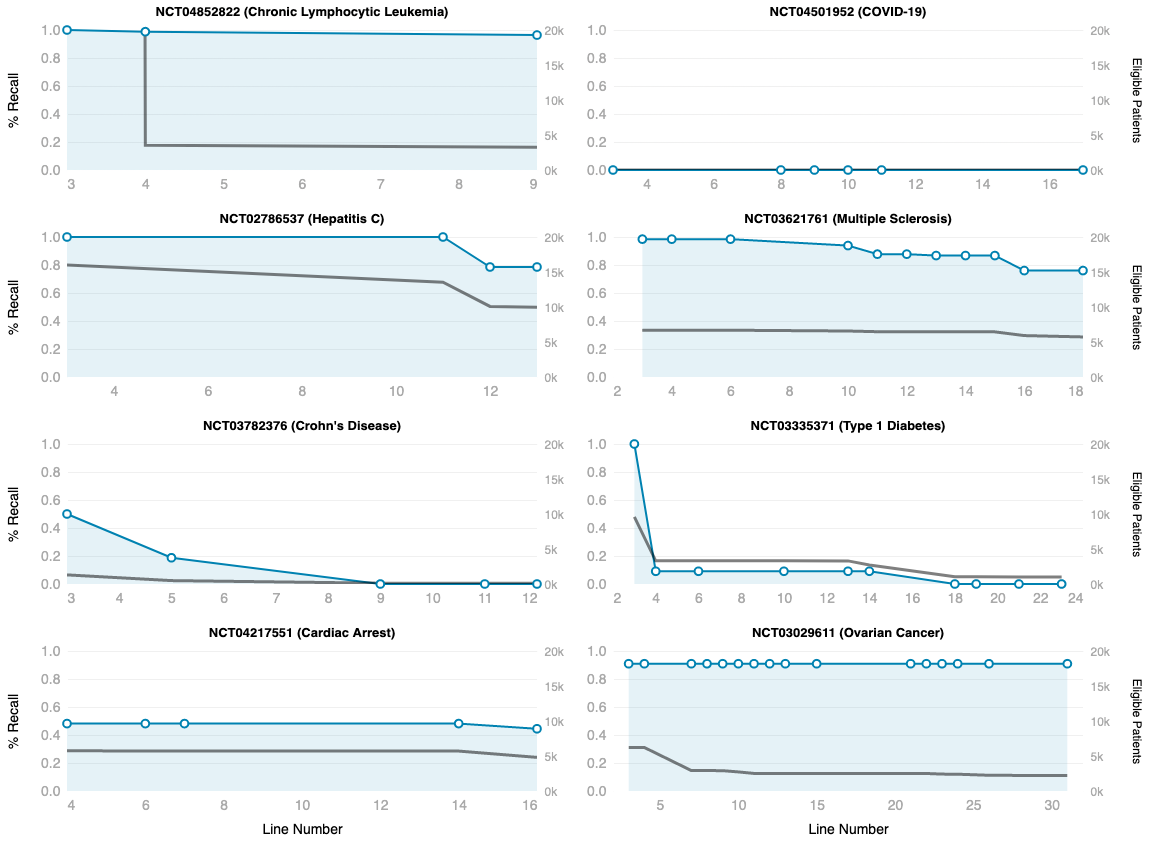
\includegraphics[scale=0.47]{Figures/Aim2/aim2_leafai_detail_results_longitudinal.png}  
  %\caption{Longitudinal results listing results of patients found at each step in the query process for each trial. The blue line indicates \% Recall (left-most Y axis) while the gray line indicates the number of eligible patients found (right-most Y axis). The X axis represents the line number within the free-text eligibility criteria. Dots indicate that the LeafAI query engine executed an eligibility criterion query.}
%\label{aim2_fig_leafai_results_detail}
%\end{figure}

Our preliminary analysis suggests a number of themes among the differing results between LeafAI and the human programmer. For example, gaps in expected data appear to result in false negatives in a number of cases. In trial NCT03335371 (Type 1 Diabetes Mellitus), one criteria specifies patients taking insulin. In the available data, however, very few enrolled patients had orders for insulin, which significantly reduced the recall of both the human programmer's and LeafAI's queries (ultimately 0\% for LeafAI, 9\% for the human programmer). We hypothesize this being due to many diabetic patients' insulin orders being performed and filled outside the UW system. Another reoccurring theme is the dual usefulness and shortcomings of LeafAI's KB. As the KB uses UMLS "is-a" parent-child concept relations to determine relevant diagnoses and so on, in many cases LeafAI casts a "wide net" and captures patients which the human programmer unintentionally does not. Conversely, the human programmer generally achieves a higher level of precision. Moreover, in certain cases the KB-determined concepts can be unhelpfully expansive. For example, in trial NCT03621761 (Multiple Sclerosis), for an exclusion criteria related to sleep disorders, LeafAI excluded eligible patients with diagnoses for drowsiness and snoring, which were likely unintended by the study investigators. We believe the latter theme speaks to the need for human review of queries, which we address in Aim 3.

\subsubsection{Limitations and Future Work}

To the best of our knowledge, the query generation and associated methods of LeafAI are the current state-of-the-art for the task of cohort discovery using a natural language interface. Nevertheless our system has a number of limitations. First, while we evaluated our query generation methods using a random sample of 8 actual clinical trials, those trials are a small subset of trials performed at the University of Washington and thus performance may vary significantly if our evaluation was expanded to a greater number of trials and disease domains. Second, while capable of reasoning across a large number of different scenarios and diseases, our KB and reasoning module use rules and pre-determined queries which likely fall short and fail to capture results in certain cases. Moreover, our reasoning module is incapable of capturing the nuance and complexities between many clinical concepts. For example, in Figure \ref{aim2_fig_leafai_querygen}, renal insufficiency and Dolutegravir are shown as contraindications to Metformin, but in reality for many patients those may not be absolute contraindications, depending on other health factors. We intend to address this by allowing users to add or remove LeafAI KB-derived concepts which they don't wish to include in Aim 3 (e.g., a user could choose to keep diagnoses of renal insufficiency while ignoring prescriptions of Dolutegravir). Last, while our logical forms representation is uniquely flexible and demonstrably capable of representing many eligibility criteria, there are nonetheless likely cases where our representation does not fully capture the semantics and nuance intended within certain criteria.

In future work, we intend to explore extending our logical form representation for general-purpose question-answering. Leveraging the outer-most functions introduced by Roberts and Demner-Fushman such as \textit{latest()}, $\lambda$\textit{()}, and \textit{min()}, our logical forms could be "wrapped" such that our logical forms are used for data retrieval while Roberts and Demner-Fushman's functions are executed to analyze returned data to answer a question. For example, the question \\

"\textit{Did the patient’s temperature exceed 38C in the last 48 hrs?}" \\

\noindent could be represented as

\begin{quote}
$\lambda( \\
    \mathrm{\ \ \ \ }measurement("temperature") \\
    \mathrm{\ \ \ \ \ \ \ }.num\_filter(eq(op(GT), val("38"), unit("C")))\\
    \mathrm{\ \ \ \ \ \ \ }.temporality(eq(op(LTEQ), val("48"), unit(HOUR))) \\
)$
\end{quote}

\noindent where the \textit{measurement()} function serves as a logical form for retrieval of relevant temperature data, while the $\lambda$\textit{()} function is executed to analyze the output and return a Boolean yes/no answer.

While general-purpose question-answering is not a specific aim of this project, the methods we have developed have potential to be a foundation for exciting future research directions. 

\subsubsection{Conclusion}

We created the LLF corpus, a gold-standard human-annotated corpus of clinical trial eligibility criteria and corresponding logical forms. The Seq2Seq model fine-tuned on this corpus achieved a relatively high BLEU score of 93.5\%. Using models trained on the LCT and LFF corpora as well as an integrated KB and other modules, we successfully developed a state-of-the-art query generation approach comparable to that of a human programmer with a mean recall of 43.5\%. Our methods in this aim enable development of the web application in Aim 3.

\end{document}